\section{Introduction}
\label{sec:intro}

\IEEEPARstart{C}{ontact}-Rich manipulation requires robots to intentionally make and break contact with objects to drive them toward desired states. Specifically, the robot needs to plan the contact sequence consisting of approaching trajectory, contact locations, contact forces, and transitions between different contact modes (i.e., contact, separation, sliding, and sticking). Such contact planning is challenging due to the combinatorial complexity of contact modes and the inherent nonsmoothness arising from the hybrid nature of contact dynamics. \textcolor{red}{Early model-based approaches typically relied on hybrid planning, either separating continuous trajectory generation from discrete contact-mode transitions through hierarchical frameworks \cite{zito2012two, wu2020r3t, haustein2015kinodynamic, chen2021trajectotree, cheng2022contact}, or handling the hybrid nature of contact with mixed-integer programs \cite{aceituno2020global, marcucci2017approximate, hogan2020feedback}.} However, this separation often suffers from poor scalability caused by the explosion of contact trajectories. Therefore, these methods offer limited manipulation strategies and poor robustness.

\textcolor{red}{
Recent advances in contact-rich manipulation have been achieved through both learning-based and model-based methods. Learning-based methods \cite{kim2023pre, lianglearning, zhou2023learning, zhang2023learning, zhou2023hacman, cho2024corn, jiang2024hacman++, le2025enhancing, lyu2025dywa} directly learn mappings from object states to contact strategies, thereby enabling complex contact-rich behaviors without explicitly modeling or optimizing through the hybrid and nonsmooth contact dynamics encountered by model-based methods. However, these methods typically rely on offline training, and their generalization is often demonstrated within specific task families, such as across unseen object geometries or variations of a predefined task. For example, DyWA \cite{lyu2025dywa} demonstrates impressive 6D non-prehensile manipulation across diverse object geometries, but remains limited to the specific robot embodiment and task on which it is trained. Consequently, achieving broadly applicable contact-rich manipulation across substantially different robot embodiments and task settings remains challenging.
}

\begin{figure}[!t]
\centerline{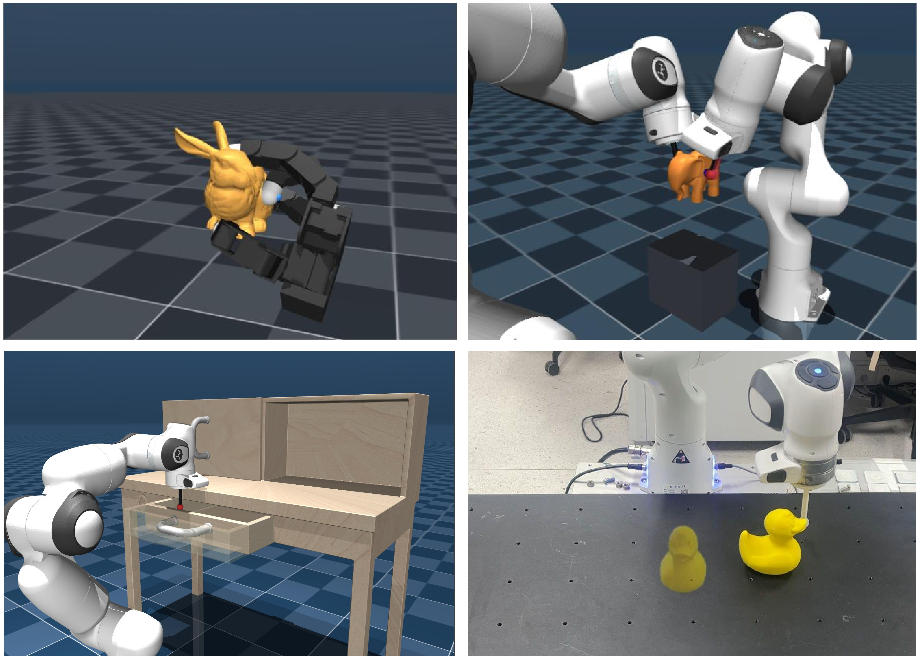
\includegraphics[width=\columnwidth]{figures/scsp_generalization.pdf}}
\caption{\textcolor{blue}{
SCSP enables online contact selection and closed-loop generation of diverse manipulation trajectories, allowing it to address a wide range of challenging contact-rich manipulation tasks.
}}
\label{fig:scsp_fig1}
\end{figure}

\begin{table*}[t]
\centering
\caption{Comparison of Contact Planning Methods.}
\label{tab:comparison}
\small
\begin{tabularx}{\textwidth}{l c c c c c}
\toprule
\textbf{Methods}
& \textbf{Perception}
& \textcolor{blue}{\textbf{Active Contact Selection}}
& \textbf{6D Manip. Exp.}
& \textbf{Real-Time}
& \textcolor{blue}{\textbf{No Obj.-Specific Analytic Geom.}} \\
\midrule

C3~\cite{aydinoglu2024consensus}
& \textcolor{blue}{Exact State}
& \ding{55}
& \ding{55}
& \ding{51}
& \ding{55} \\

CRISP~\cite{li2025surprising}
& \textcolor{blue}{Exact State}
& \textcolor{blue}{\ding{55}}
& \ding{55}
& \ding{51}
& \ding{55} \\

IDTO~\cite{kurtz2026inverse}
& \textcolor{blue}{Exact State}
& \ding{55}
& \ding{51}
& \ding{51}
& \ding{55} \\

CQDCs~\cite{pang2023global}
& \textcolor{blue}{Exact State}
& \ding{55}
& \ding{51}
& \ding{51}
& \ding{55} \\

CF-MPC~\cite{jin2024complementarity}
& \textcolor{blue}{Exact State}
& \ding{55}
& \ding{51}
& \ding{51}
& \ding{51} \\

STOCS-3D~\cite{zhang2025simultaneous}
& \textcolor{blue}{Exact State}
& \textcolor{blue}{\ding{55}}
& \ding{51}
& \ding{55}
& \ding{51} \\

\textcolor{blue}{ContactSDF~\cite{yang2024contactsdf}}
& \textcolor{blue}{Vision}
& \textcolor{blue}{\ding{55}}
& \textcolor{blue}{\ding{51}}
& \textcolor{blue}{\ding{51}}
& \textcolor{blue}{\ding{51}} \\

DyWA~\cite{lyu2025dywa}
& Vision
& \textcolor{blue}{\ding{55}}
& \ding{51}
& \ding{51}
& \ding{51} \\

Sampling~\cite{venkatesh2025approximating}
& Vision
& \ding{51}
& \ding{51}
& \ding{51}
& \ding{51} \\

\midrule

\textbf{SCSP}
& Vision
& \ding{51}
& \ding{51}
& \ding{51}
& \ding{51} \\

\bottomrule
\end{tabularx}
\end{table*}

\textcolor{red}{Contact-implicit trajectory optimization (CITO) subsequently avoids this explicit mode decomposition by modeling robot--object interaction (ROI) with complementary contact dynamics and solving the resulting trajectory optimization problem in a unified framework.}
CITO was first applied to locomotion \cite{posa2014direct, wensing2023optimization} and later extended to manipulation.
We mainly focus on Contact-Implicit Model Predictive Control (CIMPC),
\textcolor{blue}{
as its receding-horizon formulation continuously replans from the current state and is therefore particularly suitable for real-time closed-loop contact-rich manipulation.
}
\textcolor{red}{CIMPC embeds contact dynamics as constraints in a nonlinear programming (NLP) solver to compute the robot's control inputs online.}
CIMPC incorporates approximated time-stepping contact dynamics \cite{stewart2000implicit, anitescu2006optimization} into trajectory optimization, enabling online hybrid contact planning.
\textcolor{red}{Because contact models commonly used in physical simulators are often formulated as linear complementarity problems (LCPs) or quadratic programs (QPs), directly using them can hinder efficient online optimization. CIMPC methods therefore often adopt approximate contact models that trade physical fidelity for computational efficiency.}
\textcolor{blue}{
Representative methods improve the efficiency and scalability of this process through different contact-model approximations and optimization strategies \cite{aydinoglu2024consensus, pang2023global, bui2025push}. In particular, CF-MPC \cite{jin2024complementarity} introduces a complementarity-free contact model to improve the efficiency of online contact-implicit MPC, substantially accelerating contact-rich optimization.
}

\textcolor{red}{
Although CIMPC enables online planning of contact-mode transitions, actively selecting contact locations on the object remains challenging. Contact geometry and complementarity constraints make the resulting optimization nonsmooth and nonconvex, while contact-free states often provide ineffective gradients toward candidate contacts. Because contact locations are typically determined implicitly by the robot trajectory, short planning horizons and local optimization can obscure the long-term benefits of reaching distant contacts. Recent methods improve contact-rich optimization and execution: Suh et al. \cite{suh2025dexterous} introduce a contact-trust-region formulation, Jiang et al. \cite{jiang2025robust} integrate motion--contact planning with tracking, ContactSDF \cite{yang2024contactsdf} provides differentiable multi-contact models, and CRISP \cite{li2025surprising} discovers contact sequences within contact-implicit optimization. These methods, however, do not explicitly select task-relevant robot--object contact locations; CRISP is also evaluated primarily in planar settings. Venkatesh et al. \cite{venkatesh2025approximating} address this issue by sampling contact candidates and solving a local CIMPC problem for each, but at the cost of repeated lower-level optimization. Xie et al. \cite{xie2026touch} use a hierarchical RL--MPC policy to select contacts for a low-level CIMPC controller, but require task-specific training. Efficient task-directed contact selection for closed-loop planning therefore remains unresolved.
}

\textcolor{red}{
In this work, we propose Simultaneous Contact Selection and Planning (SCSP), a cascaded optimization framework for complex contact-rich manipulation. SCSP comprises Contact Selection Optimization (CSO), which performs object-centric search over candidate contact locations and provides contact guidance to steer optimization away from local optima, and Contact Planning Optimization (CPO), which plans robot actions to execute the guided contact while retaining the freedom to realize a nearby feasible contact for flexible execution. A ranking strategy couples the two modules in a cascade by comparing the CSO-guided contact with nearby candidates and passing the resulting reference to CPO.
}

\rev{Table \ref{tab:comparison} summarizes the scope of SCSP relative to representative contact-planning methods. The contributions are:}

\begin{itemize}

    \item
    \textcolor{red}{
    An efficient contact selection method, CSO, is developed for online contact-guidance generation. It samples a candidate point set and performs batched optimization to avoid direct surface-gradient search and the associated nonsmoothness of contact selection. A lightweight surrogate contact model (SCM) enables fast evaluation of candidate utility and selection of the best contact as guidance.
    }

    \item
    \textcolor{red}{
    A contact planning method, CPO, is proposed with a unified cost formulation for generating approach, contact-establishment, and contact-switching trajectories.
    }

    \item
    \textcolor{red}{
    A ranking strategy forms the cascade between contact guidance and planning by ranking the guided contact together with nearby feasible candidates. This preserves task-directed guidance while allowing CPO to select an executable nearby contact, thereby maintaining execution flexibility and contact-trajectory diversity.
    }

    \item
    \textcolor{red}{
    Extensive simulation and real-world experiments validate SCSP across diverse object geometries and contact-rich tasks. Real-world experiments further demonstrate robust vision-based nonprehensile manipulation using only simple contact calibration and without exact object perception.
    }

\end{itemize}

The rest of the paper is organized as follows. Section \ref{sec:preliminaries} reviews the preliminaries. The CSO and CPO are introduced in Sections \ref{sec:cso} and \ref{sec:cpo}, respectively. Section \ref{sec:experiment} presents the experimental results, and
\textcolor{blue}{
Section \ref{sec:generalize} evaluates structured extensions of the SCSP architecture to additional contact-rich manipulation settings.
}
Finally, discussion and limitations are presented in Section \ref{sec:discussion}, and conclusions are drawn in Section \ref{sec:conclusion}.
